\documentclass[titlepage]{article}

\usepackage{graphicx} % For images
\usepackage{float}    % For tables and other floats
\usepackage{verbatim} % For comments and other
\usepackage{amsmath}  % For math
\usepackage{amssymb}  % For more math
\usepackage{fullpage} % Set margins and place page numbers at bottom center
\usepackage{listings} % For source code
\usepackage{subfig}   % For subfigures
\usepackage[usenames,dvipsnames]{color} % For colors and names
\usepackage[hidelinks]{hyperref}           % For hyperlinks and indexing the PDF
\usepackage{libertine}
\usepackage{fontenc}
\usepackage[scaled]{beramono}
%\usepackage{lmodern}
%\usepackage{tgadventor}
\usepackage{multicol}

\hypersetup{ % play with the different link colors here
     %colorlinks = true,
     linkcolor = blue,
     frenchlinks = true
      }
      

\begin{document}


% title page/cover
\begin{titlepage}
\begin{center}

{\Huge 
Uplink User-Assisted Relaying \\ in Cellular Networks 
}~\\[4cm]

% The '~' is needed because \\ only works if a paragraph has started.

{\large 
Dual Degree Project 1st Stage Report
}~\\[2cm]

\end{center}

\begin{multicols}{2}
\begin{flushleft}
{\large
\textit{Student:} \\
\text{Prudhvi Porandla} \\
\text{110070039}
}
\end{flushleft}
\columnbreak
\begin{flushright}
{\large
\textit{Guide:} \\
\text{Prof. S. N. Merchant}
}
\end{flushright}
\end{multicols}

\vfill

\begin{center}

\includegraphics[width=4cm]{figures/iitbblack.jpg}~\\[1cm]

{\large
Department of Electrical Engineering\\
Indian Institute of Technology Bombay\\
Mumbai - 400076\\
}

\end{center}
\end{titlepage}
% cover page end
\pagenumbering{roman}


\begin{abstract}
Currently, there are 31,254 level crossings and around 40\% of them are unmanned. The unmanned
crossings are responsible for the maximum number of train accidents. The m
ain objective of this project
is to reduce the number of such accidents by building a reliable system th
at can consistently detect a train
moving towards the crossing and sets off an alarm at the crossing.
\end{abstract}


\tableofcontents
\newpage
%\mbox{}
%\newpage





\section{Introduction}
The solution to this problem is to build a system that can turn on an alarm at the crossing at least 1 min
before the train reaches the crossing and turn off the alarm when the train passes the crossing. To do this, we
designed a sensor unit, using two inductive proximity sensors, that can detect a train and its direction,
and an alarm unit. The sensor unit will be placed 1.5 km away from the crossing while the alarm unit will be
placed at the crossing. When a train passes over the two sensors of the sensor unit, it detects the direction
of the train, counts the number of axles\footnotemark\footnotetext{We actually count the number of wheels on one side, 4 wheels on each side $\implies$ 4 axles}($n$) and sends this information to the alarm unit. If the train is moving
towards the crossing, alarm unit turns on the alarm. When the train passes over the single sensor placed at the crossing,
the alarm unit down counts the number of axles from $n$ and turns off the alarm when the count reaches 0.
\\ \\
In the next sections we present the block and circuit diagrams of various units of the system, different
algorithms used to detect the direction of train and also how false alarm cases are handled.
\subsection{Motivation}
\subsection{Work Reported}
\subsection{Organization of this report}
\pagenumbering{arabic}

\section{Partial Decode-and-Forward Relaying}
In this section, we discuss the signal design, channel model and achievable rate of PDF relaying scheme.
\subsection{Signal Design}
Consider a source $\mathcal{S}$, its relay $\mathcal{R}$ and the destination $\mathcal{D}$. Each transmission block is divided into two phases: 1. broadcast transmission in which $\mathcal{S}$ broadcasts to both $\mathcal{R}$ and $\mathcal{D}$. 2. multiple access transmission in which both $\mathcal{S}$ and $\mathcal{R}$ transmit to $\mathcal{D}$. In each block of transmission, $\mathcal{S}$ splits its information into a common part and a private part. The common part is encoded via $U_s^b$ in the 1st phase and $U_s^{m_1}$ in the 2nd phase; and the private part is encoded via $V_s^{m_2}$ in the 2nd phase. The relay $\mathcal{R}$ decodes the information sent by $\mathcal{S}$ in first phase and encodes the same information using $U_s^{m_1}$ in the 2nd phase. \\ 
The signals transmitted by $\mathcal{R}$ and $\mathcal{S}$ are as follows:
\begin{align}
\text{Phase 1:}\quad x^b_s &= \sqrt{P_s^b} U_s^b, \label{eq:tranSig1}\\
\text{Phase 2:}\quad x_r^m &= \sqrt{P_r^m}U_s^{m_1}, \label{eq:tranSig2}\\ 
 x^m_s &= \sqrt{P_s^{m_1}}U_s^{m_1} + \sqrt{P_s^{m_2}}V_s^{m_2} \label{eq:tranSig3}
\end{align}
All codewords above are picked from independent Gaussian codebooks with zero mean and unit variance. \\ \\
\textbf{Power Constraints:} Let $P_s$ and $P_r$ be the transmit powers of $\mathcal{S}$ and $\mathcal{R}$ respectively and $\alpha_1$ be the fraction of transmission time allocated to first phase, then the following average power constraints should to be satisfied:
\begin{equation}
\alpha_1 P_s^b + \alpha_2 P_s^m = Ps,\quad \alpha_2P_r^m = P_r
\end{equation}
where $\alpha_2 = 1-\alpha_1$

\subsection{Channel Model}
Considering the transmit signals presented above and assuming flat fading over the two phases, the received signals at $\mathcal{R}$ and $\mathcal{D}$ during first phase are 
\begin{equation}
Y_r^b = h_{sr}x^b_s + Z_r^b , \quad Y_d^b = h_{sd}x^b_s + Z_d^b
\end{equation}
where $b$ denotes broadcast mode, $Z_r^b$ and $Z_d^b$ are \textit{i.i.d} circularly-symmetric complex gaussians with mean 0 and variance $\sigma^2$  - $\mathcal{CN}(0,\sigma^2)$ that represent noises at $\mathcal{R}$ and $\mathcal{D}$. \\
Similarly the received signal at $\mathcal{D}$ during second phase can be modelled as 
\begin{equation}
Y_d^m = h_{sd}x^m_s + h_{rd}x_r^m + Z_d^m
\end{equation}
here $m$ denotes multicast transmission; all others have usual meaning.
The above expression is true only if $\mathcal{D}$ has knowledge about the phase offset between $\mathcal{S}$ and $\mathcal{R}$. This assumption is justified by noting that the phase offset between the two nodes can be estimated at base station.

\subsection{Achievable Rate}
With transmit signals in equations~\ref{eq:tranSig1}-~\ref{eq:tranSig3} and joint ML decoding rule at $\mathcal{D}$, the achievable rate for this relaying scheme is:
\begin{equation} \label{eq:rate}
R_{PDF} \leq min(C_1+C_2,C_3)
\end{equation}
\begin{align}
\text{where } C_1 &= \alpha_1 \log\Big(1+|h_{sr}|^2P_s^b\Big),\\
C_2 &= \alpha_2 \log\Big(1+|h_{sd}|^2P_s^{m_2}\Big),\\
C_3 &= \alpha_1 \log\Big(1+|h_{sd}|^2P_s^b\Big) + \alpha_2\log\bigg(1+|h_{sd}|^2P_s^{m_2} + \Big(|h_{sd}|\sqrt{P_s^{m_1}} + |h_{rd}|\sqrt{P_r^m}\Big)^2\bigg)
\end{align}
$C_1$ represents the rate of the common part that can be decoded at $\mathcal{R}$, $C_2$  the private part that can be decoded at $\mathcal{D}$ provided the common part has been decoded correctly, and $C_3$ both the common and private parts that can be jointly decoded at $\mathcal{D}$. These rates are achievable provided full CSIR at all receivers and the source-relay phase offset knowledge.
\par
Now that we know what PDF relaying scheme is and the achievable rate, let us see how this scheme performs in cellular networks. To analyse system performance under PDF relaying, we need to know network geometry i.e., how the users and base stations are distributed, how many users can take advantage of relaying, how users identify a potential relay etc. In the next couple of sections we describe network geometry,  received signals and interference model when relaying is deployed in the whole network, and cooperation policies.

\section{Cellular Network Geometry and User-Assisted Relaying}

\subsection{Network geometry model}
Consider a cellular system which consists of multiple
cells, each cell has a single base station and each base station
serves multiple users. Each of the users uses a distinct frequency
block. Each user is served by the single base station that
is closest to that user.

\begin{figure}[H]
\begin{center}
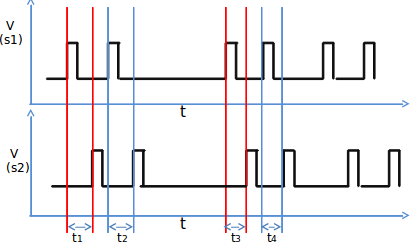
\includegraphics[height = 2in,width=4in,angle=00]{figures/8w_no_miss.png}
\caption{\small pulses on s1, s2 as train crosses the sensor unit}
\label{fig:sysModel}
\end{center}
\end{figure}

\par We use stochastic geometry to
describe the uplink cellular network as shown in Fig.~\ref{fig:sysModel}. We
assume that the active users in different cells that use the same resource block and cause interference to each other are distributed on a two-dimensional plane according to a homogeneous and stationary Poisson point process (PPP)
$\Phi_1$ with intensity $\lambda_1$. The set of user equipments(UEs) that are in idle state and can participate in relaying are distributed according to another PPP $\Phi_2$ with intensity $\lambda_2$. We assume $\Phi_1$ and $\Phi_2$ are independent. Furthermore, under the assumption that each BS serves a
single mobile in a given resource block, the BS should be closer to its served UE than to any other UE. Therefore we assume each BS is uniformly distributed in the Voronoi cell of its served UE. Fig.~\ref{fig:netLayout} shows an example layout of the model.

\begin{figure}[H]
\begin{center}
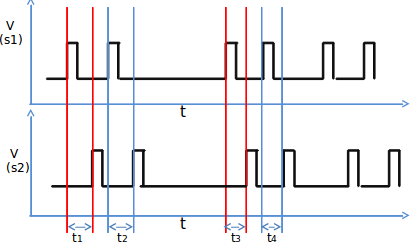
\includegraphics[height = 2in,width=4in,angle=00]{figures/8w_no_miss.png}
\caption{\small pulses on s1, s2 as train crosses the sensor unit}
\label{fig:netLayout}
\end{center}
\end{figure}

\subsection{Channel Model}
In this section, we describe the channel model when PDF relaying is deployed in cellular network. In this case, there will be out-of-cell inteference in addition to noise. The interference is due to frequency reuse in other cells.
\par Consider $i^{th}$ cell, we model the received signals at the relay and base station in this cell during 1st phase as
\begin{equation*}
Y_{r,i}^b = h^{(i)}_{sr}x_{s,i}^b + I_{r,i}^b + Z_{r,i}^b,
\end{equation*}
\begin{equation}
Y_{d,i}^b = h^{(i)}_{sd}x_{s,i}^b + I_{d,i}^b + Z_{d,i}^b
\end{equation}
where $I_{r,i}^b$ and $I_{d,i}^b$ represent the interference received at the $i^{th}$ relay and destination. 
\par 
In second phase of the transmission, the received signal at the BS can be modelled as 
\begin{equation}
Y_{d,i}^m = h^{(i)}_{sd}x_{s,i}^m + h^{(i)}_{rd}x_{r,i}^m+ I_{d,i}^m + Z_{d,i}^m
\end{equation}

\subsection{Interference}
To model interference, we assume prefect frame synchronization. LTE-Advanced imposes very strict requirements on synchronization anyway. Interference at the relay during first phase and at the destination(BS) during first and second phases can be expressed as
\begin{equation*}
I_{r,i}^b = \sum_{k \neq i} B_k h^{(k,i)}_{sr} x_{s,k}^b + (1-B_k)h_{sr}^{(k,i)}x_{s,k} ,
\end{equation*}
\begin{equation*}
I_{d,i}^b = \sum_{k \neq i} B_k h_{sd}^{(k,i)} x^b_{s,k} + (1-B_k)h_{sd}^{(k,i)}x_{s,k},
\end{equation*}
\begin{equation} \label{eq:interferences}
I_{d,i}^m = \sum_{k \neq i} B_k \Big(h_{sd}^{(k,i)} x^m_{s,k} + h_{rd}^{(k,i)} x^m_{r,k}\Big) + (1-B_k)h_{sd}^{(k,i)}x_{s,k}
\end{equation}
the summation is over all active users. Here, $h_{sd}^{(k,i)}$ and $h_{rd}^{(k,i)}$ , respectively, are the channel fading from the $k^{th}$ active UE in $\Phi_1$ and the associated relaying UE in $\Phi_2$ to the BS associated with the $i^{th}$ active UE in $\Phi_1$; and $h_{sr}^{(k,i)}$ is the channel fading from the $k^{th}$ active UE in $\Phi_1$ to the relaying UE associated with the $i^{th}$ active UE in $\Phi_1$.
\par $B_k$ in above expressions is a Bernoulli random variable with success probability $\rho$. $B_k = 1$ is used to indicate the $k^{th}$ active UE's decision to exploit the help of another idle UE, a relay, and apply the relaying transmission strategy, and $B_k = 0$ indicates that the $k^{th}$ UE has no relay. In section~\ref{sec:coop}, we derive the cooperation probability $\rho$ for different cooperation policies.
\par
 For a given setting of nodes locations, based on the
interference model in Eq.~\ref{eq:interferences}, we can use the fact
that interference at either the relay or destination is the
sum of an infinite number of signals undergoing independent fading from nodes distributed in the infinite 2-D plane and use the law of large numbers to approximate the interference as a complex Gaussian distribution.
Also, since the transmitted codewords complex Gaussian with zero mean, mean of interference is zero. To fully characterize interference as a
complex Gaussian distribution, we define their distributions as $ I_{d,i}^b \sim \mathcal{CN} (0,\mathcal{Q}_{d,i}^b), I_{d,i}
^m \sim \mathcal{CN}(0,\mathcal{Q}_{d,i}^m),$ and $I_{r,i}^b \sim \mathcal{CN}
(0,\mathcal{Q}_{r,i})$ with the variances derived later
in Section~\ref{sec:interference}. The power of these interference terms which
correspond to the variance of the Gaussian random variables
are function of node locations and hence vary with different
network realizations.

\subsection{Equivalent Standard Channel Model}
Using the interference model discussed above, we can convert the channel model in case of relaying into the standard form to capture the effects of
interference into the channel fading as
\begin{align*}
\tilde{Y}_{r,i}^b &= \tilde{h}_{sr}^{(i)}x_{s,i}^b + \tilde{Z}_{r,i}^b, \\
\tilde{Y}_{d,i}^b &= \tilde{h}_{sd}^{(i)}x_{s,i}^b + \tilde{Z}_{d,i}^b, \\
\tilde{Y}_{d,i}^m &= \tilde{h}_{sd}^{(i)}x_{s,i}^m + \tilde{h}_{rd}^{(i)}x_{r,i}^m + \tilde{Z}_{d,i}^m
\end{align*}
where the new channel fading terms are defined as

\begin{equation*}
\tilde{h}_{sr}^{(i)} = \frac{h_{sr}^{(i)}}{\sqrt{\mathcal{Q}_{r,i} + \sigma^2}}, \quad \tilde{h}_{sd}^{(b,i)} = \frac{h_{sd}^{(i)}}{\sqrt{\mathcal{Q}_{d,i}^b + \sigma^2}} \quad
\tilde{h}_{sd}^{(m,i)} = \frac{h_{sd}^{(i)}}{\sqrt{\mathcal{Q}_{d,i}^m + \sigma^2}},
\quad \tilde{h}_{rd}^{(i)} = \frac{h_{rd}^{(i)}}{\sqrt{\mathcal{Q}_{d,i}^m + \sigma^2}}
\end{equation*}
and the noise terms are now all $\mathcal{CN}(0,1)$. Using these equivalent 
standard channels, we can compute the transmission rate as in Eq.~\ref{eq:rate}

\section{Cooperation Policies and Probability} \label{sec:coop}
In this section, we look at three cooperation policies: an ideal policy $E_1$, a 
pure geometric policy $E_2$ and a hybrid policy $E_3$ that defines whether an active UE should select an inactive UE to use it in PDF relaying. Also, expressions for cooperation probabilities of $E_2$ and $E_3$ are derived.
\subsection{Policies}
\subsubsection{Ideal Policy $E_1$}
The ideal cooperation policy $E_1$ requires the active UE nodes to know instantaneous  SINRs of the relay link($\mathcal{S}-\mathcal{R}$) and the
direct link($\mathcal{S}-\mathcal{D}$). The policy is defined as 
\begin{align*}
E_1 &= \Big\{|\tilde{h}_{(sr)}^{(k)}|^2 \geq |\tilde{h}_{(sd)}^{(k)}|^2\Big\} \\
&\backsimeq \Big\{ \frac{g_{sr}r_2^{-\alpha}}{\mathcal{Q}_{r,k}} \geq \frac{g_{sd}r_1^{-\alpha}}{\mathcal{Q}_{d,k}^b} \Big\}
\end{align*}
where $r_1$ and $r_2$ denote the direct distance
between $\mathcal{S}$ and $\mathcal{D}$ and cooperation distance between $\mathcal{S}$ and its closest idle UE, respectively and $\alpha$ is pathloss exponent. This event $E_1$ identifies whether an idle UE will be associated as a relay for the $k^{th}$ UE and participate in transmission. Noise variance $\sigma^2$ is ignored since interference dominates. 
\par Since interference at relay and destination during first phase is more or less the same and $g_{sr}, g_{sd}$ are identically distributed, we can safely ignore them and propose a policy that depends only on distances.

\subsubsection{Pure Geometric Policy $E_2$}
This policy is defined as
\begin{equation}
E_2 = \{r_2\leq r_1, D \leq r_1 \}
\end{equation}
where $D$ is the distance between $\mathcal{R}$ and $\mathcal{D}$. In words, if source's(active UE's) nearest idle neighbour is in the intersection region of two circles of radius $r_1$ centered at source and destination, then that idle UE will be chosen to act as a relay.
\par $E_2$ is more practical than policy $E_1$ in the sense that
it does not require full knowledge of both the channel fading
and the interference at the decision making node. Instead, it
only requires the decision making nodes to know the distances
from the active user to the nearest idle user and to the base
station. It represents a practical decision making strategy for
fast fading channels, requiring no knowledge of the channel
fading. 
\subsubsection{Hybrid Policy $E_3$}
This policy is proposed for slow fading channels where small scale fading parameters estimation and their
feedback to the decision making node is feasible. 
\begin{equation}
E_3 = \{g_{sd}r_1^{-\alpha} \leq g_{sr}r_2^{-\alpha}, D \leq r_1 \}
\end{equation}
Note that this cooperation policy is still independent of the
interference as in the pure geometric cooperation policy $E_2$.




\section{Interference Analysis} \label{sec:interference}

\section{Simulations and Results}

\section{Conclusions and Future Work}

\section{References}

\end{document}
